\section{Requirements}

\subsection{Minimum viable product (MVP)}

\noindent A minimum viable product (MVP) is a version of the saman application which includes the features that will allow to release the product to a small group of test users by solving the core problem for these sets of users. The purpose is to provide immediate value, quickly, while minimizing development costs.\\

\noindent A common misconception is that an MVP consists of the minimum set of features deemed necessary for a working software product, with the goal of bringing it to market quickly. This misses the mark on several levels, most notably in the over-emphasis on speedy delivery and time to market, as opposed to focusing on customer and market acceptance. Indeed, rapid development is of essence, but only to the extent that learning and research objectives can be obtained quickly. Accordingly, some of the noted purposes of an MVP below begin to open up a more significant discussion:
\begin{itemize}
    \item Be able to test a product hypothesis with minimal resources
    \item Accelerate learning
    \item Reduce wasted engineering hours
    \item Get the product to early customers as soon as possible 
\end{itemize}

\noindent Accordingly, in terms of the saman application the MVP serves as a common ground to reach agreement on the implementation of the requirements left for the final version of the application. All the source code related to the saman application is to be published and accessed through the saman Central Github Repository.\\

\noindent In the preceding subsection (section \ref{subsec:overall_workflow}), an overall workflow in the MVP is presented which provide the software developers the information they need to set up the saman working product. A list of future requirements are also presented in subsection \ref{subsec:future_req}. We need to emphasize that the requirements listed in subsection \ref{subsec:future_req} are not included as they fall outside the scope of this MVP.

\subsection{Overall workflow}
\label{subsec:overall_workflow}

\noindent A decision was made to create a simple MVP in order to make it easier for users and potential business partners to understand, download and test the saman application for the  transportation of goods in the goods markets of Pakistan. The overall workflow of the saman application is created by the project and can be used by users and all stakeholders to get an overview and supply feedback to the development team to solve their specific issues. It can also be used by any who are interested in details about the saman project.\\

\noindent The saman application contain a number of views (\texttt{screens}) which the project has agreed to be included in the MVP. The overall workflow includes the following \texttt{screens}:
\begin{itemize}
    \item \texttt{SplashScreen}: This is the landing page that links to the \texttt{WelcomeScreen};
    \item \texttt{WelomeScreen}: Contains buttons that allow the user to choose to either \texttt{SignInWithPhoneNumber}, \texttt{SignInWithFacebook}, \texttt{SignInWithGoogle}, \texttt{SignInWithEmail}, \texttt{SignUpIfNoAccount};
    \item \texttt{LanguageScreen}: As it is assumed that users may not speak English, this \texttt{screen} will allow the users to select between the two default languages in the application, i.e. English or Urdu;
    \item \texttt{PhoneLoginScreen}: The users use this \texttt{screen} to login with the default method, i.e. with phone number;
    \item \texttt{SignUpWithEmailScreen}: Should the user not have an account, this can be created in this \texttt{screen} with an email; 
    \item \texttt{EmailLoginScreen}: The users use this \texttt{screen} to login with the default method, i.e. email. This assumes that the user already has an account in the application;
    \item \texttt{SelectionScreen (reDirectWrapper)}; When creating an account the users is asked to choose to be a customer or driver. This selection is done in this \texttt{screeen} and the \texttt{screen} re-directs the users to one of two preceding \texttt{screens};
    \item \texttt{DriverHomeScreen}: This \texttt{screen} is reserved for users with driver account. As a minimum this \texttt{screen} should include a list of all the open possible orders (\texttt{ListOfOrders}) that the driver can choose to pursue; 
    \item \texttt{CustomerHomeScreen}: Assuming that the user is sign-in as an customer, this screen allows the users to select \texttt{From}, \texttt{To} and the \texttt{SizeOfObject} that they which to transport; 
\end{itemize}

\noindent The overall workflow is illustrated in Figure \ref{fig:overall_flow}.

\subsection{Future requirements}
\label{subsec:future_req}

\noindent As part of discussions within the project team, a list of possible future features is attached below. It needs to be emphasized that this part of the document is an evolving part, i.e. team members are recommended to contact the author whenever new or changes to future requirements are introduced.
\begin{itemize}
    \item \textbf{Cost-effective zones}: This future requirement involves showing drivers recommended areas that are more cost-effective, i.e. areas with high demand, but without sufficient number of drivers to satisfy the demand.
    \item \textbf{Drill-down areas}: In addition for drivers and customers to select district polygons in map. It should be possible to select sub-districts as a way to "drill-down" areas in order to specify a trip more accurately. This is done as full address information may not be available at all times and for all users.
    \item \textbf{Dynamic pricing}: This requirement includes the possibility to set prices of a trip based on the supply and demand, i.e. high demand should transfer to higher prices and vice-versa. This is done to incentive driver to use the saman platform.
    \item \textbf{Real-time database}
\end{itemize}

\begin{figure}


\tikzset{every picture/.style={line width=0.75pt}} %set default line width to 0.75pt        

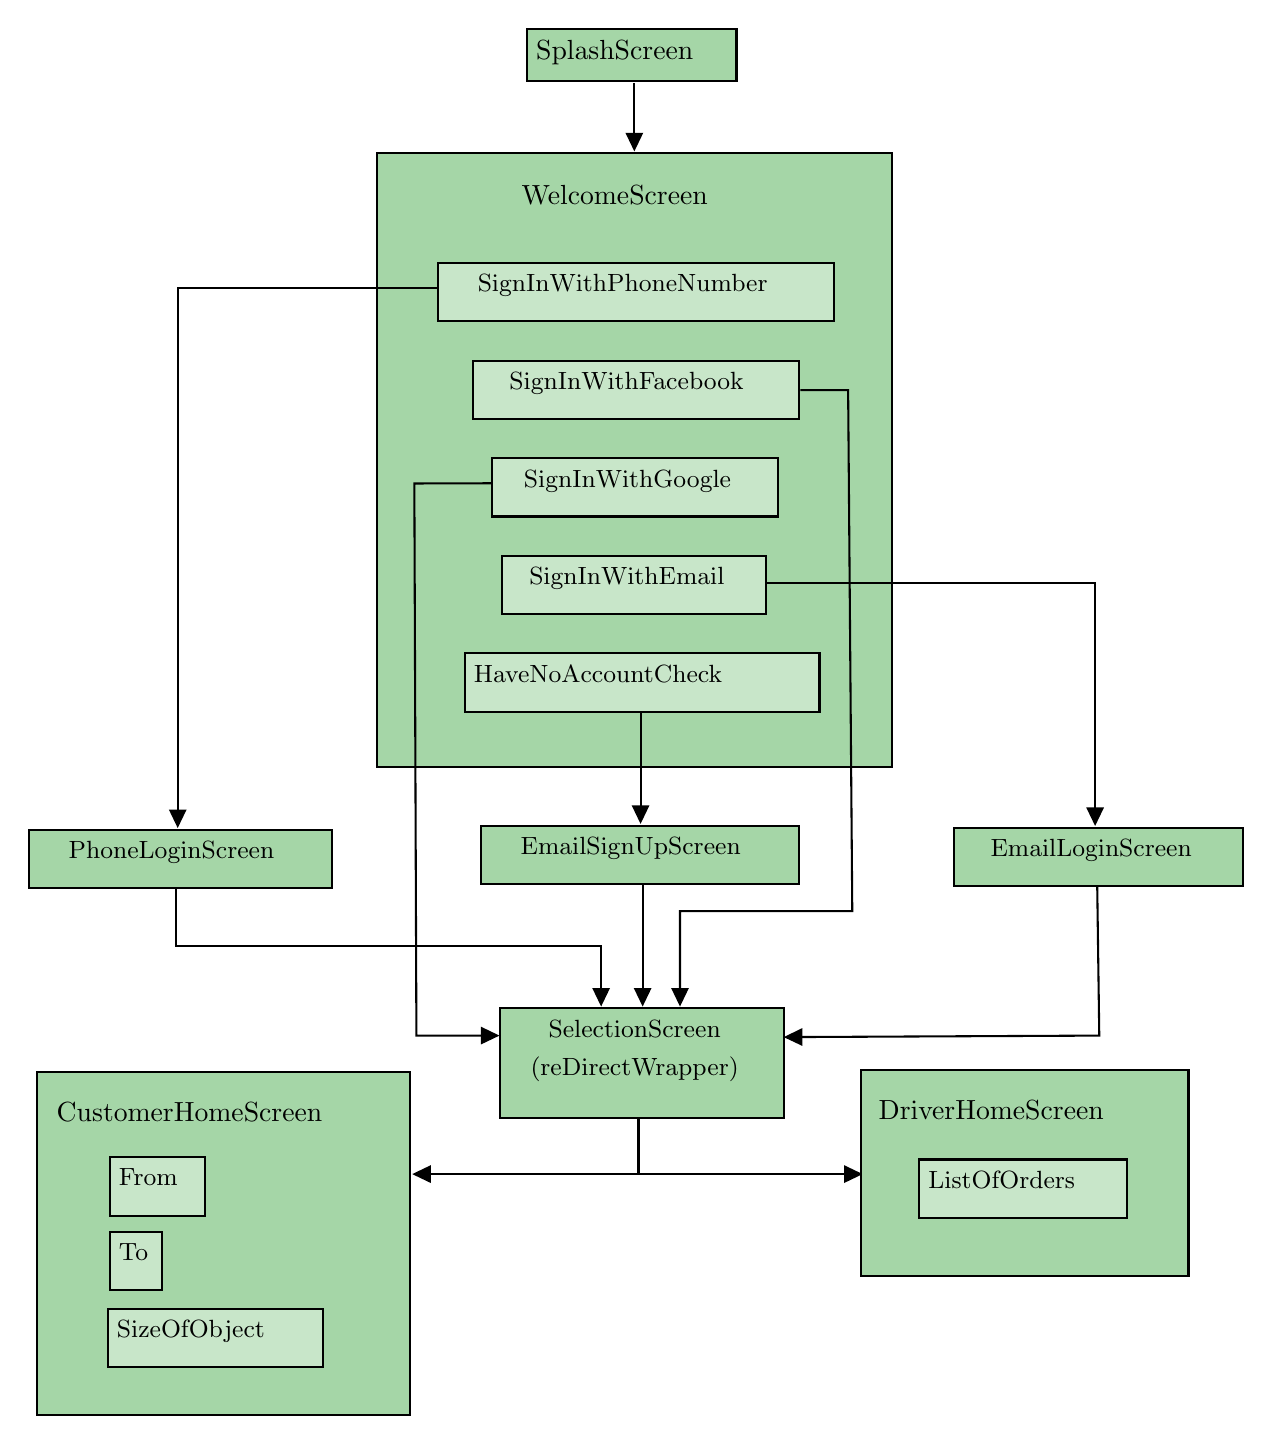
\begin{tikzpicture}[x=0.75pt,y=0.75pt,yscale=-1,xscale=1]
%uncomment if require: \path (0,739); %set diagram left start at 0, and has height of 739

%Straight Lines [id:da7113497462701521] 
\draw    (335.79,44.11) -- (335.79,74.11) ;
\draw [shift={(335.79,77.11)}, rotate = 270] [fill={rgb, 255:red, 0; green, 0; blue, 0 }  ][line width=0.08]  [draw opacity=0] (8.93,-4.29) -- (0,0) -- (8.93,4.29) -- cycle    ;
%Shape: Rectangle [id:dp804679553514686] 
\draw  [fill={rgb, 255:red, 165; green, 214; blue, 167 }  ,fill opacity=1 ] (211.79,78) -- (459.79,78) -- (459.79,373.61) -- (211.79,373.61) -- cycle ;
%Straight Lines [id:da7748155015830069] 
\draw    (241.79,143.11) -- (115.79,143.11) -- (115.79,400.11) ;
\draw [shift={(115.79,403.11)}, rotate = 270] [fill={rgb, 255:red, 0; green, 0; blue, 0 }  ][line width=0.08]  [draw opacity=0] (8.93,-4.29) -- (0,0) -- (8.93,4.29) -- cycle    ;
%Straight Lines [id:da7985297999599543] 
\draw    (399.79,285.11) -- (557.79,285.11) -- (557.79,399.11) ;
\draw [shift={(557.79,402.11)}, rotate = 270] [fill={rgb, 255:red, 0; green, 0; blue, 0 }  ][line width=0.08]  [draw opacity=0] (8.93,-4.29) -- (0,0) -- (8.93,4.29) -- cycle    ;
%Straight Lines [id:da7337816453122255] 
\draw    (267,237) -- (229.79,237.11) -- (230.79,503.11) -- (267.79,503.11) ;
\draw [shift={(270.79,503.11)}, rotate = 180] [fill={rgb, 255:red, 0; green, 0; blue, 0 }  ][line width=0.08]  [draw opacity=0] (8.93,-4.29) -- (0,0) -- (8.93,4.29) -- cycle    ;
%Straight Lines [id:da284513979563384] 
\draw    (415.79,192.11) -- (438.79,192.11) -- (440.79,443.11) -- (357.79,443.11) -- (357.79,486.11) ;
\draw [shift={(357.79,489.11)}, rotate = 270] [fill={rgb, 255:red, 0; green, 0; blue, 0 }  ][line width=0.08]  [draw opacity=0] (8.93,-4.29) -- (0,0) -- (8.93,4.29) -- cycle    ;
%Straight Lines [id:da546691753229293] 
\draw    (114.79,430.11) -- (114.79,460.11) -- (319.79,460.11) -- (319.79,486.11) ;
\draw [shift={(319.79,489.11)}, rotate = 270] [fill={rgb, 255:red, 0; green, 0; blue, 0 }  ][line width=0.08]  [draw opacity=0] (8.93,-4.29) -- (0,0) -- (8.93,4.29) -- cycle    ;
%Straight Lines [id:da2721201746016835] 
\draw    (558.79,430.11) -- (559.79,503.11) -- (410.79,503.83) ;
\draw [shift={(407.79,503.84)}, rotate = 359.73] [fill={rgb, 255:red, 0; green, 0; blue, 0 }  ][line width=0.08]  [draw opacity=0] (8.93,-4.29) -- (0,0) -- (8.93,4.29) -- cycle    ;
%Straight Lines [id:da9264108411386227] 
\draw    (338.79,346.11) -- (338.79,398.11) ;
\draw [shift={(338.79,401.11)}, rotate = 270] [fill={rgb, 255:red, 0; green, 0; blue, 0 }  ][line width=0.08]  [draw opacity=0] (8.93,-4.29) -- (0,0) -- (8.93,4.29) -- cycle    ;
%Straight Lines [id:da2580705187866017] 
\draw    (339.79,430.11) -- (339.79,486.11) ;
\draw [shift={(339.79,489.11)}, rotate = 270] [fill={rgb, 255:red, 0; green, 0; blue, 0 }  ][line width=0.08]  [draw opacity=0] (8.93,-4.29) -- (0,0) -- (8.93,4.29) -- cycle    ;
%Straight Lines [id:da6089173734133702] 
\draw    (337.79,518.84) -- (337.79,569.84) -- (231.79,569.84) ;
\draw [shift={(228.79,569.84)}, rotate = 360] [fill={rgb, 255:red, 0; green, 0; blue, 0 }  ][line width=0.08]  [draw opacity=0] (8.93,-4.29) -- (0,0) -- (8.93,4.29) -- cycle    ;
%Straight Lines [id:da35122879335401014] 
\draw    (337.79,569.84) -- (442.79,569.84) ;
\draw [shift={(445.79,569.84)}, rotate = 180] [fill={rgb, 255:red, 0; green, 0; blue, 0 }  ][line width=0.08]  [draw opacity=0] (8.93,-4.29) -- (0,0) -- (8.93,4.29) -- cycle    ;
%Shape: Rectangle [id:dp36316864788775893] 
\draw  [fill={rgb, 255:red, 165; green, 214; blue, 167 }  ,fill opacity=1 ] (47.79,520.82) -- (227.79,520.82) -- (227.79,685.84) -- (47.79,685.84) -- cycle ;
%Shape: Rectangle [id:dp5437324655273716] 
\draw  [fill={rgb, 255:red, 165; green, 214; blue, 167 }  ,fill opacity=1 ] (445,519.82) -- (602.79,519.82) -- (602.79,618.75) -- (445,618.75) -- cycle ;

% Text Node
\draw  [fill={rgb, 255:red, 165; green, 214; blue, 167 }  ,fill opacity=1 ]  (284,18) -- (385,18) -- (385,43) -- (284,43) -- cycle  ;
\draw (287,22) node [anchor=north west][inner sep=0.75pt]   [align=left] {SplashScreen};
% Text Node
\draw (280,92) node [anchor=north west][inner sep=0.75pt]   [align=left] {WelcomeScreen};
% Text Node
\draw  [fill={rgb, 255:red, 200; green, 230; blue, 201 }  ,fill opacity=1 ]  (241,131) -- (432,131) -- (432,159) -- (241,159) -- cycle  ;
\draw (244,135) node [anchor=north west][inner sep=0.75pt]  [font=\large] [align=left] {\begin{minipage}[lt]{127.00768000000002pt}\setlength\topsep{0pt}
\begin{center}
{\small SignInWithPhoneNumber}
\end{center}

\end{minipage}};
% Text Node
\draw  [fill={rgb, 255:red, 200; green, 230; blue, 201 }  ,fill opacity=1 ]  (258,178) -- (415,178) -- (415,206) -- (258,206) -- cycle  ;
\draw (261,182) node [anchor=north west][inner sep=0.75pt]  [font=\large] [align=left] {\begin{minipage}[lt]{104.35688000000002pt}\setlength\topsep{0pt}
\begin{center}
{\small SignInWithFacebook}
\end{center}

\end{minipage}};
% Text Node
\draw  [fill={rgb, 255:red, 200; green, 230; blue, 201 }  ,fill opacity=1 ]  (267,225) -- (405,225) -- (405,253) -- (267,253) -- cycle  ;
\draw (270,229) node [anchor=north west][inner sep=0.75pt]  [font=\large] [align=left] {\begin{minipage}[lt]{91.50080000000001pt}\setlength\topsep{0pt}
\begin{center}
{\small SignInWithGoogle}
\end{center}

\end{minipage}};
% Text Node
\draw  [fill={rgb, 255:red, 200; green, 230; blue, 201 }  ,fill opacity=1 ]  (272,272) -- (399,272) -- (399,300) -- (272,300) -- cycle  ;
\draw (275,276) node [anchor=north west][inner sep=0.75pt]  [font=\large] [align=left] {\begin{minipage}[lt]{83.52236pt}\setlength\topsep{0pt}
\begin{center}
{\small SignInWithEmail}
\end{center}

\end{minipage}};
% Text Node
\draw  [fill={rgb, 255:red, 165; green, 214; blue, 167 }  ,fill opacity=1 ]  (44,404) -- (190,404) -- (190,432) -- (44,432) -- cycle  ;
\draw (47,408) node [anchor=north west][inner sep=0.75pt]  [font=\large] [align=left] {\begin{minipage}[lt]{96.41720000000001pt}\setlength\topsep{0pt}
\begin{center}
{\small PhoneLoginScreen}
\end{center}

\end{minipage}};
% Text Node
\draw  [fill={rgb, 255:red, 165; green, 214; blue, 167 }  ,fill opacity=1 ]  (490,403) -- (629,403) -- (629,431) -- (490,431) -- cycle  ;
\draw (493,407) node [anchor=north west][inner sep=0.75pt]  [font=\large] [align=left] {\begin{minipage}[lt]{92.10940000000002pt}\setlength\topsep{0pt}
\begin{center}
{\small EmailLoginScreen}
\end{center}

\end{minipage}};
% Text Node
\draw  [fill={rgb, 255:red, 165; green, 214; blue, 167 }  ,fill opacity=1 ]  (271,490) -- (408,490) -- (408,543) -- (271,543) -- cycle  ;
\draw (274,494) node [anchor=north west][inner sep=0.75pt]  [font=\large] [align=left] {\begin{minipage}[lt]{90.6508pt}\setlength\topsep{0pt}
\begin{center}
{\small SelectionScreen }\\{\small (reDirectWrapper)}
\end{center}

\end{minipage}};
% Text Node
\draw  [fill={rgb, 255:red, 200; green, 230; blue, 201 }  ,fill opacity=1 ]  (254,319) -- (425,319) -- (425,347) -- (254,347) -- cycle  ;
\draw (257,323) node [anchor=north west][inner sep=0.75pt]  [font=\large] [align=left] {{\small HaveNoAccountCheck}};
% Text Node
\draw  [fill={rgb, 255:red, 165; green, 214; blue, 167 }  ,fill opacity=1 ]  (262,402) -- (415,402) -- (415,430) -- (262,430) -- cycle  ;
\draw (265,406) node [anchor=north west][inner sep=0.75pt]  [font=\large] [align=left] {\begin{minipage}[lt]{101.28532000000001pt}\setlength\topsep{0pt}
\begin{center}
{\small EmailSignUpScreen}
\end{center}

\end{minipage}};
% Text Node
\draw (56,533.82) node [anchor=north west][inner sep=0.75pt]   [align=left] {CustomerHomeScreen};
% Text Node
\draw (452,532.82) node [anchor=north west][inner sep=0.75pt]   [align=left] {DriverHomeScreen};
% Text Node
\draw  [fill={rgb, 255:red, 200; green, 230; blue, 201 }  ,fill opacity=1 ]  (83,561.82) -- (129,561.82) -- (129,589.82) -- (83,589.82) -- cycle  ;
\draw (86,565.82) node [anchor=north west][inner sep=0.75pt]  [font=\large] [align=left] {{\small From}};
% Text Node
\draw  [fill={rgb, 255:red, 200; green, 230; blue, 201 }  ,fill opacity=1 ]  (83,597.82) -- (108,597.82) -- (108,625.82) -- (83,625.82) -- cycle  ;
\draw (86,601.82) node [anchor=north west][inner sep=0.75pt]  [font=\large] [align=left] {{\small To}};
% Text Node
\draw  [fill={rgb, 255:red, 200; green, 230; blue, 201 }  ,fill opacity=1 ]  (82,634.82) -- (186,634.82) -- (186,662.82) -- (82,662.82) -- cycle  ;
\draw (85,638.82) node [anchor=north west][inner sep=0.75pt]  [font=\large] [align=left] {{\small SizeOfObject}};
% Text Node
\draw  [fill={rgb, 255:red, 200; green, 230; blue, 201 }  ,fill opacity=1 ]  (473,562.82) -- (573,562.82) -- (573,590.82) -- (473,590.82) -- cycle  ;
\draw (476,566.82) node [anchor=north west][inner sep=0.75pt]  [font=\large] [align=left] {{\small ListOfOrders}};


\end{tikzpicture}
    
\caption{MVP overall workflow}
\label{fig:overall_flow}
\end{figure}